%definira klasu dokumenta 
\documentclass[12pt]{report} 

%prostor izmedu naredbi \documentclass i \begin{document} se zove uvod. U njemu se nalaze naredbe koje se odnose na cijeli dokument

%osnovni LaTex ne može riješiti sve probleme, pa se koriste različiti paketi koji olakšavaju izradu željenog dokumenta
\usepackage[croatian]{babel} 
\usepackage{amssymb}
\usepackage{amsmath}
\usepackage{txfonts}
\usepackage{mathdots}
\usepackage{titlesec}
\usepackage{array}
\usepackage{lastpage}
\usepackage{etoolbox}
\usepackage{tabularray}
\usepackage{color, colortbl}
\usepackage{adjustbox}
\usepackage{geometry}
\usepackage[classicReIm]{kpfonts}
\usepackage{hyperref}
\usepackage{fancyhdr}

\usepackage{float}
\usepackage{setspace}
\restylefloat{table}


\patchcmd{\chapter}{\thispagestyle{plain}}{\thispagestyle{fancy}}{}{} %redefiniranje stila stranice u paketu fancyhdr

%oblik naslova poglavlja
\titleformat{\chapter}{\normalfont\huge\bfseries}{\thechapter.}{20pt}{\Huge}
\titlespacing{\chapter}{0pt}{0pt}{40pt}


\linespread{1.3} %razmak između redaka

\geometry{a4paper, left=1in, top=1in,}  %oblik stranice

\hypersetup{ colorlinks, citecolor=black, filecolor=black, linkcolor=black,	urlcolor=black }   %izgled poveznice


%prored smanjen između redaka u nabrajanjima i popisima
\newenvironment{packed_enum}{
	\begin{enumerate}
		\setlength{\itemsep}{0pt}
		\setlength{\parskip}{0pt}
		\setlength{\parsep}{0pt}
	}{\end{enumerate}}

\newenvironment{packed_item}{
	\begin{itemize}
		\setlength{\itemsep}{0pt}
		\setlength{\parskip}{0pt}
		\setlength{\parsep}{0pt}
	}{\end{itemize}}




%boja za privatni i udaljeni kljuc u tablicama
\definecolor{LightBlue}{rgb}{0.9,0.9,1}
\definecolor{LightGreen}{rgb}{0.9,1,0.9}

%Promjena teksta za dugačke tablice
\DefTblrTemplate{contfoot-text}{normal}{Nastavljeno na idućoj stranici}
\SetTblrTemplate{contfoot-text}{normal}
\DefTblrTemplate{conthead-text}{normal}{(Nastavljeno)}
\SetTblrTemplate{conthead-text}{normal}
\DefTblrTemplate{middlehead,lasthead}{normal}{Nastavljeno od prethodne stranice}
\SetTblrTemplate{middlehead,lasthead}{normal}

%podesavanje zaglavlja i podnožja

\pagestyle{fancy}
\lhead{Programsko inženjerstvo}
\rhead{ParkShare}
\lfoot{Proggers}
\cfoot{stranica \thepage/\pageref{LastPage}}
\rfoot{\today}
\renewcommand{\headrulewidth}{0.2pt}
\renewcommand{\footrulewidth}{0.2pt}


\begin{document} 
	
	
	
	\begin{titlepage}
		\begin{center}
			\vspace*{\stretch{1.0}} %u kombinaciji s ostalim \vspace naredbama definira razmak između redaka teksta
			\LARGE Programsko inženjerstvo\\
			\large Ak. god. 2020./2021.\\
			
			\vspace*{\stretch{3.0}}
			
			\huge ParkShare\\
			\Large Dokumentacija, Rev. 1\\
			
			\vspace*{\stretch{12.0}}
			\normalsize
			Grupa: Proggers\\
			Voditelj: Marko Barbir\\
			
			
			\vspace*{\stretch{1.0}}
			Datum predaje: 17.11.2021.\\
	
			\vspace*{\stretch{4.0}}
			
			Nastavnik: Hrvoje Nuić, mag. ing.\\
		
		\end{center}

	
	\end{titlepage}

	
	\tableofcontents


	\chapter{Dnevnik promjena dokumentacije}
		
		\textbf{\textit{Kontinuirano osvježavanje}}\\
				
		
		\begin{longtabu} to \textwidth {|X[2, l]|X[13, l]|X[3, l]|X[3, l]|}
			\hline \multicolumn{1}{|l|}{\textbf{Rev.}}	& \multicolumn{1}{l|}{\textbf{Opis promjene/dodatka}} & \multicolumn{1}{|l|}{\textbf{Autori}} & \multicolumn{1}{l|}{\textbf{Datum}} \\[3pt] \hline
			\endfirsthead
			
			\hline \multicolumn{1}{|l|}{\textbf{Rev.}}	& \multicolumn{1}{l|}{\textbf{Opis promjene/dodatka}} & \multicolumn{1}{|l|}{\textbf{Autori}} & \multicolumn{1}{l|}{\textbf{Datum}} \\[3pt] \hline
			\endhead
			
			\hline 
			\endlastfoot
			
			0.1 & Napravljen predložak.	& Ivošević & 22.08.2013. 		\\[3pt] \hline 
			0.2	& Dopisane upute za povijest dokumentacije.\newline Dodane reference. & Jović & 24.08.2013. 	\\[3pt] \hline 
			0.5 & Dodan \textit{Use Case} dijagram i jedan sekvencijski dijagram, funkcionalni i nefunkcionalni zahtjevi i dodatak A & Ivošević & 25.08.2013. \\[3pt] \hline 
			0.6 & Arhitektura i dizajn sustava, algoritmi i strukture podataka & Grudenić & 26.08.2013. \\[3pt] \hline 
			0.8 & Povijest rada i trenutni status implementacije,\newline Zaključci i plan daljnjeg rada & Ivošević & 28.08.2013. \\[3pt] \hline 
			0.9 & Opisi obrazaca uporabe & Jović & 07.09.2013. \\[3pt] \hline 
			0.10 & Preveden uvod & Jović & 08.09.2013. \\[3pt] \hline 
			0.11 & Sekvencijski dijagrami & Žužak & 09.09.2013. \\[3pt] \hline 
			0.12.1 & Započeo dijagrame razreda & Horvat & 10.09.2013. \\[3pt] \hline 
			0.12.2 & Nastavak dijagrama razreda & Horvat & 11.09.2013. \\[3pt] \hline 
			\textbf{1.0} & Verzija samo s bitnim dijelovima za 1. ciklus & Ivošević & 11.09.2013. \\[3pt] \hline 
			1.1 & Uređivanje teksta -- funkcionalni i nefunkcionalni zahtjevi & Grudenić \newline Jović & 14.09.2013. \\[3pt] \hline 
			1.2 & Manje izmjene:Timer - Brojilo vremena & Grudenić & 15.09.2013. \\[3pt] \hline 
			1.3 & Popravljeni dijagrami obrazaca uporabe & Jović & 15.09.2013. \\[3pt] \hline 
			1.5 & Generalna revizija strukture dokumenta & Ivošević & 19.09.2013. \\[3pt] \hline 
			1.5.1 & Manja revizija (dijagram razmještaja) & Jović & 20.09.2013. \\[3pt] \hline 
			\textbf{2.0} & Konačni tekst predloška dokumentacije  & Ivošević & 28.09.2013. \\[3pt] \hline 
			&  &  & \\[3pt] \hline
			
			
		\end{longtabu}
	
	
		\textit{Moraju postojati glavne revizije dokumenata 1.0 i 2.0 na kraju prvog i drugog ciklusa. Između tih revizija mogu postojati manje revizije već prema tome kako se dokument bude nadopunjavao. Očekuje se da nakon svake značajnije promjene (dodatka, izmjene, uklanjanja dijelova teksta i popratnih grafičkih sadržaja) dokumenta se to zabilježi kao revizija. Npr., revizije unutar prvog ciklusa će imati oznake 0.1, 0.2, …, 0.9, 0.10, 0.11.. sve do konačne revizije prvog ciklusa 1.0. U drugom ciklusu se nastavlja s revizijama 1.1, 1.2, itd.}
	\chapter{Opis projektnog zadatka}
		
		\textbf{\textit{dio 1. revizije}}\\
		
		\textit{Na osnovi projektnog zadatka detaljno opisati korisničke zahtjeve. Što jasnije opisati cilj projektnog zadatka, razraditi problematiku zadatka, dodati nove aspekte problema i potencijalnih rješenja. Očekuje se minimalno 3, a poželjno 4-5 stranica opisa.	Teme koje treba dodatno razraditi u ovom poglavlju su:}
		\begin{packed_item}
			\item \textit{potencijalna korist ovog projekta}
			\item \textit{postojeća slična rješenja (istražiti i ukratko opisati razlike u odnosu na zadani zadatak). Dodajte slike koja predočavaju slična rješenja.}
			\item \textit{skup korisnika koji bi mogao biti zainteresiran za ostvareno rješenje.}
			\item \textit{mogućnost prilagodbe rješenja }
			\item \textit{opseg projektnog zadatka}
			\item \textit{moguće nadogradnje projektnog zadatka}
		\end{packed_item}
		
		\textit{Za pomoć pogledati reference navedene u poglavlju „Popis literature“, a po potrebi konzultirati sadržaj na internetu koji nudi dobre smjernice u tom pogledu.}
		\eject
		
		\section{Primjeri u \LaTeX u}
		
		\textit{Ovo potpoglavlje izbrisati.}\\

		U nastavku se nalaze različiti primjeri kako koristiti osnovne funkcionalnosti \LaTeX a koje su potrebne za izradu dokumentacije. Za dodatnu pomoć obratiti se asistentu na projektu ili potražiti upute na sljedećim web sjedištima:
		\begin{itemize}
			\item Upute za izradu diplomskog rada u \LaTeX u - \url{https://www.fer.unizg.hr/_download/repository/LaTeX-upute.pdf}
			\item \LaTeX\ projekt - \url{https://www.latex-project.org/help/}
			\item StackExchange za Tex - \url{https://tex.stackexchange.com/}\\
		
		\end{itemize} 	


		
		\noindent \underbar{podcrtani tekst}, \textbf{podebljani tekst}, 	\textit{nagnuti tekst}\\
		\noindent \normalsize primjer \large primjer \Large primjer \LARGE {primjer} \huge {primjer} \Huge primjer \normalsize
				
		\begin{packed_item}
			
			\item  primjer
			\item  primjer
			\item  primjer
			\item[] \begin{packed_enum}
				\item primjer
				\item[] \begin{packed_enum}
					\item[1.a] primjer
					\item[b] primjer
				\end{packed_enum}
				\item primjer
			\end{packed_enum}
			
		\end{packed_item}
		
		\noindent primjer url-a: \url{https://www.fer.unizg.hr/predmet/proinz/projekt}
		
		\noindent posebni znakovi: \# \$ \% \& \{ \} \_ 
		$|$ $<$ $>$ 
		\^{} 
		\~{} 
		$\backslash$ 
		
		
		\begin{longtblr}[
			label=none,
			entry=none
			]{
				width = \textwidth,
				colspec={|X[8,l]|X[8, l]|X[16, l]|}, 
				rowhead = 1,
			} %definicija širine tablice, širine stupaca, poravnanje i broja redaka naslova tablice
			\hline \multicolumn{3}{|c|}{\textbf{naslov unutar tablice}}	 \\ \hline[3pt]
			\SetCell{LightGreen}IDKorisnik & INT	&  	Lorem ipsum dolor sit amet, consectetur adipiscing elit, sed do eiusmod  	\\ \hline
			korisnickoIme	& VARCHAR &   	\\ \hline 
			email & VARCHAR &   \\ \hline 
			ime & VARCHAR	&  		\\ \hline 
			\SetCell{LightBlue} primjer	& VARCHAR &   	\\ \hline 
		\end{longtblr}
		

		\begin{longtblr}[
				caption = {Naslov s referencom izvan tablice},
				entry = {Short Caption},
			]{
				width = \textwidth, 
				colspec = {|X[8,l]|X[8,l]|X[16,l]|}, 
				rowhead = 1,
			}
			\hline
			\SetCell{LightGreen}IDKorisnik & INT	&  	Lorem ipsum dolor sit amet, consectetur adipiscing elit, sed do eiusmod  	\\ \hline
			korisnickoIme	& VARCHAR &   	\\ \hline 
			email & VARCHAR &   \\ \hline 
			ime & VARCHAR	&  		\\ \hline 
			\SetCell{LightBlue} primjer	& VARCHAR &   	\\ \hline 
		\end{longtblr}
	


		
		
		%unos slike
		\begin{figure}[H]
			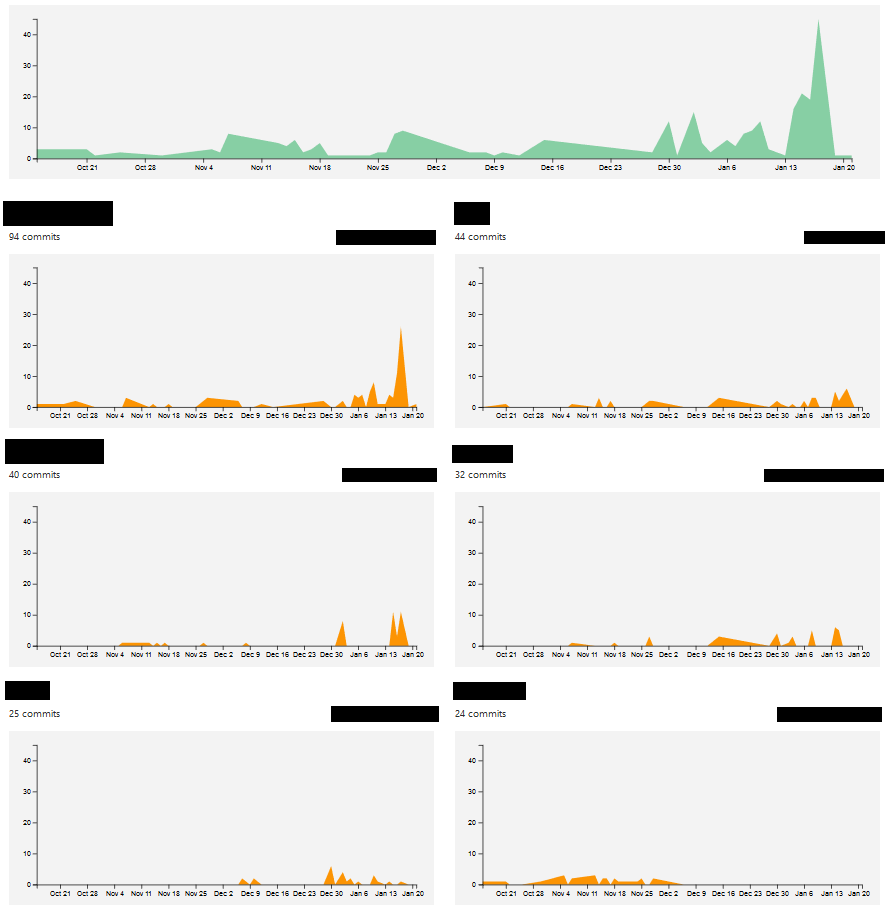
\includegraphics[scale=0.4]{slike/aktivnost.PNG} %veličina slike u odnosu na originalnu datoteku i pozicija slike
			\centering
			\caption{Primjer slike s potpisom}
			\label{fig:promjene}
		\end{figure}
		
		\begin{figure}[H]
			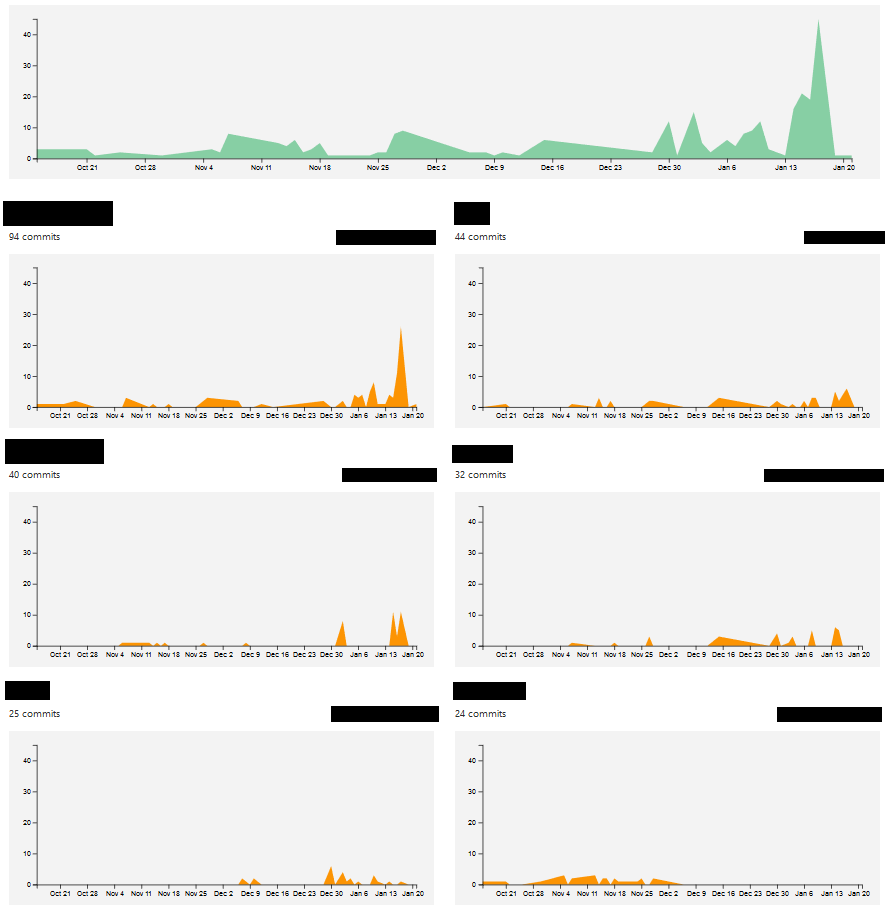
\includegraphics[width=\textwidth]{slike/aktivnost.PNG} %veličina u odnosu na širinu linije
			\caption{Primjer slike s potpisom 2}
			\label{fig:promjene2} %label mora biti drugaciji za svaku sliku
		\end{figure}
		
		Referenciranje slike \ref{fig:promjene2} u tekstu.
		
		\eject
		
	
	\chapter{Specifikacija programske potpore}
		
	\section{Funkcionalni zahtjevi}
			
			\textbf{\textit{dio 1. revizije}}\\
			
			\textit{Navesti \textbf{dionike} koji imaju \textbf{interes u ovom sustavu} ili  \textbf{su nositelji odgovornosti}. To su prije svega korisnici, ali i administratori sustava, naručitelji, razvojni tim.}\\
				
			\textit{Navesti \textbf{aktore} koji izravno \textbf{koriste} ili \textbf{komuniciraju sa sustavom}. Oni mogu imati inicijatorsku ulogu, tj. započinju određene procese u sustavu ili samo sudioničku ulogu, tj. obavljaju određeni posao. Za svakog aktora navesti funkcionalne zahtjeve koji se na njega odnose.}\\
			
			
			\noindent \textbf{Dionici:}
			
			\begin{packed_enum}
				
				\item Asistent (Naručitelj)
				\item Korisnici				
				\item Vlasnici parkinga
				\item Administrator(i)
				\item Razvojni tim
				
			\end{packed_enum}
			
			\noindent \textbf{Aktori i njihovi funkcionalni zahtjevi:}
			
			
			\begin{packed_enum}
				\item  \underbar{Vlasnik parkinga (inicijator) može:}
				
				\begin{packed_enum}
					
					\item Napraviti (max 1) parkiralište, te ga izbrisati, ili promijeniti ime i cjenik
					\item Ucrtati nova i izbrisati postojeća parking mjesta za svoj parking
					\item Definirati i promijeniti mogućnost rezervacije pojedinog parkirališnog mjesta
					\item Pregledati svoje osobne podatke i promijeniti ih
					\item Izbrisati svoj korisnički račun
					\item Pregledati statistiku zauzetosti svog parkirališta i parkirališnih mjesta kroz vrijeme u obliku grafa
					
				\end{packed_enum}
			
				\item  \underbar{ Neregistrirani/neprijavljeni korisnik (inicijator) može:}
				
				\begin{packed_enum}
					
					\item Registrirati se kao klijent ili kao vlasnik parkinga
					\item Prijaviti se
					\item Pregledati sva parkirališta i parkirališna mjesta dostupna u aplikaciji
					
				\end{packed_enum}
			
				\item  \underbar{Prijavljeni klijent (inicijator) može:}
				
				\begin{packed_enum}
					
					\item Odjaviti se
					\item Pregledati svoje osobne podatke i promijeniti ih
					\item izbrisati korisnički račun
					\item Pregledati sva parkirališta i parkirališna mjesta dostupna u aplikaciji te njihovu zauzetost u realnom vremenu i rezervati ih
					\item Upisati destinaciju, tip prijevoza i procjenu trajanja parkinga te dobiti mogućnost rezervacije najbližeg parkirališnog mjesta
					\item Uplatiti novac u račun
					\item Pregledati povijest transakcija i rezervacija
					
				\end{packed_enum}
			
				\item  \underbar{Administrator (inicijator) može:}
				
				\begin{packed_enum}
					
					\item Odjaviti se
					\item Izbrisati ili promijeniti korisnički račun bilo kojeg ne-administratorskog korisnika
					\item Pregledati sva parkirališta i parkirališna mjesta dostupna u aplikaciji, te promijeniti njihove podatke
					\item Potvrditi novi račun vlasnika parkirališta
					
				\end{packed_enum}
			
				\item  \underbar{Baza podataka (sudionik):}
				
				\begin{packed_enum}
					
					\item Pohranjuje sve podatke o korisnicima i njihovim ovlastima
					\item Pohranjuje sve podatke o parkiralištima (ime, cjenik)
					\item Pohranjuje sve podatke o parkirališnim mjestima (zauzetost, tip)
					
				\end{packed_enum}
			
				\item  \underbar{Senzor zauzetosti (inicijator):}
				
				\begin{packed_enum}
					
					\item Šalje signal kad se parkirališno mjesto zauzme ili oslobodi
					
				\end{packed_enum}
			\end{packed_enum}
			
			\eject 
			
			
				
			\subsection{Obrasci uporabe}
				
				\subsubsection{Opis obrazaca uporabe}
			
					\noindent \underbar{\textbf{UC1 - Dodavanje parkirališta}}
					\begin{packed_item}
						
						\item \textbf{Glavni sudionik: }\text{Voditelj parkirališta}
						\item  \textbf{Cilj:} \text{Dodavanje parkirališta u bazu podataka}
						\item  \textbf{Sudionici:} \text{Voditelj parkirališta, baza podataka}
						\item  \textbf{Preduvjet:} \text{Korisnik mora imati ulogu voditelja parkinga}
						\item  \textbf{Opis osnovnog tijeka:}
						
						\item[] \begin{packed_enum}
							
							\item \text{Voditelj parkirališta odabire opciju za dodavanje parkinga}							
							\item \text{Voditelj parkirališta unosi informacije o svom parkiralištu}							
							\item \text{Voditelj parkirališta na karti unosi dostupna parkirališna mjesta}							
													
							\item \text{Voditelj parkirališta postavlja senzor koji osvježava informaciju zauzetosti parkirališnog mjesta}						
						\end{packed_enum}
						
						\item  \textbf{Opis mogućih odstupanja:}
						
						\item[] \begin{packed_item}
							
							\item[2.a] Unešeno već postojeće ime parkinga
							\item[] \begin{packed_enum}
								
								\item Aplikacija ispisuje grešku
								
							\end{packed_enum}
							\item[3.a] Označavanje mjesta na karti na kojem već postoji parking
							\item[] \begin{packed_enum}
								
								\item Aplikacija ispisuje grešku
								
							\end{packed_enum}
							\item[4.a] Aplikacija se ne može povezati sa senzorom
							\item[] \begin{packed_enum}
								
								\item Aplikacija ispisuje grešku
								
							\end{packed_enum}
							
						\end{packed_item}
					\end{packed_item}
					\noindent \underbar{\textbf{UC2 - Brisanje parkirališta}}
					\begin{packed_item}
						
						\item \textbf{Glavni sudionik: }Voditelj parkirališta
						\item  \textbf{Cilj:} Brisanje parkirališta
						\item  \textbf{Sudionici:} Voditelj parkirališta, baza podataka
						\item  \textbf{Preduvjet:} Korisnik mora imati ulogu voditelja parkinga, voditelj mora upravljati tim parkingom, parkiralište već postoji u bazi podataka
						\item  \textbf{Opis osnovnog tijeka:}
						
						\item[] \begin{packed_enum}
							
							
							\item Voditelj zatraži brisanje parkirališta
							\item Parkiralište se briše iz baze podataka
							\item Voditelju se javlja da je parkiralište uspješno izbrisano
							
						\end{packed_enum}
						
						\item  \textbf{Opis mogućih odstupanja:}
						
						\item[] \begin{packed_item}
							
							\item[2.a] Neuspješno brisanje podataka iz baze podataka	
							\item[] \begin{packed_enum}
								
								\item Aplikacija ispisuje grešku
								
							\end{packed_enum}
						\end{packed_item}
					\end{packed_item}
				    \noindent \underbar{\textbf{UC3 - Izmjena podataka o parkiralištu}}
				   \begin{packed_item}
				   	
				   	\item \textbf{Glavni sudionik: }Voditelj parkirališta
				   	\item  \textbf{Cilj:} Izmjena podataka o parkiralištu
				   	\item  \textbf{Sudionici:} Voditelj parkirališta, baza podataka
				   	\item  \textbf{Preduvjet:} Korisnik mora imati ulogu voditelja parkinga, voditelj mora upravljati tim parkingom, parkiralište već postoji u bazi podataka
				   	\item  \textbf{Opis osnovnog tijeka:}
				   	
				   	\item[] \begin{packed_enum}
				   		
				   		\item Voditelj zatraži izmjenu podataka
				   		\item Voditelj unosi nove izmjenjene podatke o parkiralištu
				   		\item Novi podatci se spremaju u bazu podataka
				   		\item Voditelju se javlja da su podatci uspješno izmjenjeni
				   	\end{packed_enum}
				   	
				   	\item  \textbf{Opis mogućih odstupanja:}
				   	
				   	\item[] \begin{packed_item}
				   		
				   		
				   		
				   		\item[3.a] Neuspješno spremanje podataka u bazu podataka	
				   		\item[] \begin{packed_enum}
				   			
				   			\item Aplikacija ispisuje grešku
				   			
				   		\end{packed_enum}
				   		
				   	\end{packed_item}
				   \end{packed_item}
			    	\noindent \underbar{\textbf{UC4 - Izmjena podataka o parkirališnom mjestu}}
			    	\begin{packed_item}
			    		
			    		\item \textbf{Glavni sudionik: }Voditelj parkirališta
			    		\item  \textbf{Cilj:} Izmjena podataka o parkirališnom mjestu
			    		\item  \textbf{Sudionici:} Voditelj parkirališta, baza podataka
			    		\item  \textbf{Preduvjet:} Korisnik mora imati ulogu voditelja parkinga, voditelj mora upravljati tim parkingom, parkiralište i parkirno mjesto već postoji u bazi podataka
			    		\item  \textbf{Opis osnovnog tijeka:}
			    		
			    		\item[] \begin{packed_enum}
			    			
			    			\item Voditelj zatraži izmjenu podataka
			    			\item Voditelj unosi nove izmjenjene podatke o parkirališnom mjestu
			    			\item Novi podatci se spremaju u bazu podataka
			    			\item Voditelju se javlja da su podatci uspješno izmjenjeni
			    		\end{packed_enum}
			    		
			    		\item  \textbf{Opis mogućih odstupanja:}
			    		
			    		\item[] \begin{packed_item}
			    			\item[3.a] Neuspješno spremanje podataka u bazu podataka	
			    			\item[] \begin{packed_enum}
			    				
			    				\item Aplikacija ispisuje grešku
			    				
			    			\end{packed_enum}
			    			
			    	\end{packed_item}
		    		\noindent \underbar{\textbf{UC5 - Dodavanje parkirališnog mjesta}}
		    		\begin{packed_item}
		    			\item \textbf{Glavni sudionik: }Voditelj parkirališta
		    			\item  \textbf{Cilj:} Dodavanje parkirališnog mjesta
		    			\item  \textbf{Sudionici:} Voditelj parkirališta, baza podataka
		    			\item  \textbf{Preduvjet:} Korisnik mora imati ulogu voditelja parkinga, voditelj mora upravljati tim parkingom, parkiralište i parkirno mjesto već postoji u bazi podataka
		    			\item  \textbf{Opis osnovnog tijeka:}
		    			
		    			\item[] \begin{packed_enum}
		    				
		    				\item Voditelj zatraži dodavanje novog parkirališnog mjesta na parkiralištu
		    				\item Voditelj na karti ucrtaje parkirališno mjesto
		    				\item Voditelj parkirališta definira je li moguće rezervirati parkirališno mjesto
		    				\item Podatci se spremaju u bazu podataka
		    				\item Voditelju se javlja da su podatci uspješno spremljeni u bazi podataka
		    			\end{packed_enum}
		    			
		    			\item  \textbf{Opis mogućih odstupanja:}
		    			
		    			\item[] \begin{packed_item}
		    				
		    				\item[2.a] Voditelj dodaje parkirališno mjesto na lokaciji na kojoj vec postoji parkirališno mjesto
		    				\item[] \begin{packed_enum}
		    					
		    					\item Voditelja se upozorava o grešci
		    					
		    				\end{packed_enum}
	    				
	    				\item[4.a] Neuspješno spremanje podataka u bazu podataka	
	    				\item[] \begin{packed_enum}
	    					
	    					\item Aplikacija ispisuje grešku
	    					
	    				\end{packed_enum}
		    				
		    			\end{packed_item}
		    		\end{packed_item}
	    			\noindent \underbar{\textbf{UC6 - Brisanje parking mjesta}}
	    			\begin{packed_item}
	    				
	    				\item \textbf{Glavni sudionik: }Voditelj parkirališta
	    				\item  \textbf{Cilj:} Brisanje parking mjesta
	    				\item  \textbf{Sudionici:} Voditelj parkirališta, baza podataka
	    				\item  \textbf{Preduvjet:} Korisnik mora imati ulogu voditelja parkinga, voditelj mora upravljati tim parkingom, parkiralište već postoji u bazi podataka
	    				\item  \textbf{Opis osnovnog tijeka:}
	    				
	    				\item[] \begin{packed_enum}
	    					
	    					\item Voditelj zatraži brisanje parkiraling mjesta
	    					\item Parkirališno mjesto se briše iz baze podataka
	    					\item Voditelju se javlja da je parkiralište uspješno izbrisano
	    				\end{packed_enum}
	    				
	    				\item  \textbf{Opis mogućih odstupanja:}
	    				
	    				\item[] \begin{packed_item}
	    					
	    					\item[2.a] Neuspješno brisanje podataka iz baze podataka	
	    					\item[] \begin{packed_enum}
	    						
	    						\item Aplikacija ispisuje grešku
	    						
	    					\end{packed_enum}
	    				\end{packed_item}
	    			\end{packed_item}
    				\noindent \underbar{\textbf{UC7 - Definiranje mogućnosti rezervacije pojedinog parkirališnog mjesta}}
    				\begin{packed_item}
    					
    					\item \textbf{Glavni sudionik: }Voditelj parkirališta
    					\item  \textbf{Cilj:} Definiranje mogućnosti rezervacije pojedinog parkirališnog mjesta
    					\item  \textbf{Sudionici:} Voditelj parkirališta, baza podataka
    					\item  \textbf{Preduvjet:} Korisnik mora imati ulogu voditelja parkinga, voditelj mora upravljati tim parkingom, parkiralište već postoji u bazi podataka
    					\item  \textbf{Opis osnovnog tijeka:}
    					
    					\item[] \begin{packed_enum}
    						
    						\item Voditelj odabire parkirališno mjesto 
    						\item Voditelj definira mogućnost rezervacije parkirališnog mjesta
    						\item Informacije se spremaju u bazi podataka
    						\item Voditelju se javlja da su podatci uspješno spremljeni
    					
    					\end{packed_enum}
    					
    					\item  \textbf{Opis mogućih odstupanja:}
    					
    					\item[] \begin{packed_item}
    						
    						\item[3.a] Neuspješno spremanje podataka u bazu podataka	
    						\item[] \begin{packed_enum}
    							
    							\item Aplikacija ispisuje grešku
    							
    						\end{packed_enum}
    						
    					\end{packed_item}
    				\end{packed_item}
    				\noindent \underbar{\textbf{UC8 - Promjena mogućnosti rezervacije pojedinog parkirališnog mjesta}}
    				\begin{packed_item}
    					
    					\item \textbf{Glavni sudionik:} Senzor zauzetosti
    					\item  \textbf{Cilj:} Omogućuje ponovnu rezervaciju novog tek oslobođenog mjesta
    					\item  \textbf{Sudionici:} Baza podataka
    					\item  \textbf{Preduvjet:} 
    					\item  \textbf{Opis osnovnog tijeka:}
    					
    					\item[] \begin{packed_enum}
    						
    						\item Vozilo dođe ili ode sa parkirališnog mjesta
    						\item Senzor registrira promjenu
    						\item Promjena se pohranjuje u bazu podataka
    					\end{packed_enum}
    					
    					\item  \textbf{Opis mogućih odstupanja:}
    					
    					\item[] \begin{packed_item}
    						
    						\item[2.a] Kvar na senzoru zauzetosti
    						\item[] \begin{packed_enum}
    							
    							\item Hitan popravak ili zamjena senzora od strane vlasnika parkinga
    							
    						\end{packed_enum}
    						
    					\end{packed_item}
    				\end{packed_item}
    			
    				\noindent \underbar{\textbf{UC9 - Pregled osobnih podataka}}
    				\begin{packed_item}
    					
    					\item \textbf{Glavni sudionik:} Administrator
    					\item  \textbf{Cilj:} Dati administratoru posebnu mogućnost pregleda osobnih podataka svih registriranih korisnika
    					\item  \textbf{Sudionici:} Baza podataka
    					\item  \textbf{Preduvjet:} Glavni sudionik nužno mora biti prijavljen kao administrator
    					\item  \textbf{Opis osnovnog tijeka:}
    					
    					\item[] \begin{packed_enum}
    						
    						\item Administrator zatraži pregled osobnih podataka određenog registriranog korisnika
    						\item Određeni podaci se dohvaćaju iz baze podataka
    						\item Podaci se formatirano prikazuju administratoru
    					\end{packed_enum}
    					
    					\item  \textbf{Opis mogućih odstupanja:}
    					
    					\item[] \begin{packed_item}
    						
    						\item[2.a] Neuspjelo dohvaćanje podataka iz baze podataka
    						\item[] \begin{packed_enum}
    							
    							\item Aplikacija ispisuje grešku
    							
    						\end{packed_enum}
    						
    					\end{packed_item}
    				\end{packed_item}
    				\noindent \underbar{\textbf{UC10 - Promjena osobnih podataka}}
    				\begin{packed_item}
    					
    					\item \textbf{Glavni sudionik:} Administrator
    					\item  \textbf{Cilj:} Dati administratoru posebnu mogućnost izmjene osobnih podataka svih registriranih korisnika
    					\item  \textbf{Sudionici:} Baza podataka
    					\item  \textbf{Preduvjet:} Glavni sudionik nužno mora biti prijavljen kao administrator
    					\item  \textbf{Opis osnovnog tijeka:}
    					
    					\item[] \begin{packed_enum}
    						
    						\item Administrator zatraži pregled osobnih podataka određenog registriranog korisnika
    						\item Određeni podaci se dohvaćaju iz baze podataka
    						\item Administrator odluči mijenjati osobne podatke odabranog korisnika
    						\item Administrator potvrdi promjene
    						\item Promjene se pohranjuju u bazu podataka
    					\end{packed_enum}
    					
    					\item  \textbf{Opis mogućih odstupanja:}
    					
    					\item[] \begin{packed_item}
    						
    						\item[2.a] Neuspjelo dohvaćanje podataka iz baze podataka
    						\item[] \begin{packed_enum}
    							
    							\item Aplikacija ispisuje grešku
    							
    						\end{packed_enum}
    						\item[3.a] Administrator je unio krivi format podataka
    						\item[] \begin{packed_enum}
    							
    							\item Aplikacija upozorava na krivi format i ne dopušta potvrdu
    							
    						\end{packed_enum}
    						\item[5.a] Neuspjela pohrana u bazu podataka
    						\item[] \begin{packed_enum}
    							
    							\item Aplikacija ispisuje grešku
    							
    						\end{packed_enum}
    						
    					\end{packed_item}
    				\end{packed_item}
    				\noindent \underbar{\textbf{UC11 - Registracija u sustav}}
    			\begin{packed_item}
    				
    				\item \textbf{Glavni sudionik:} Neregistrirani korisnik 
    				\item  \textbf{Cilj:} Omogućuje neregistriranom korisniku registraciju u sustav
    				\item  \textbf{Sudionici:} Baza podataka
    				\item  \textbf{Preduvjet:} Glavni sudionik nije registriran od prije
    				\item  \textbf{Opis osnovnog tijeka:}
    				
    				\item[] \begin{packed_enum}
    					
    					\item Neregistrirani korisnik šalje zahtjev za registraciju sa određenom ulogom za koju se hoće prijaviti (voditelj parkinga ili klijent)
    					\item Neregistrirani korisnik upisuje potrebne podatke (ime, prezime email,...)
    					\item Neregistrirani korisnik potvrđuje svoje podatke
    					\item Ako se korisnik prijavio kao voditelj parkinga administrator ga mora potvrditi
    					\item Podaci o novoregistriranom korisniku se pohranjuju u bazu podataka
    					\item Registracija se završava potvrdom preko email adrese
    				\end{packed_enum}
    				
    				\item  \textbf{Opis mogućih odstupanja:}
    				
    				\item[] \begin{packed_item}
    					
    					\item[2.a] Upisani podaci nisu u pravilnom formatu
    					\item[] \begin{packed_enum}
    						
    						\item Aplikacija upozorava na krivi format i ne dopušta nastavak
    						
    					\end{packed_enum}
    					\item[5.a] Neuspjela pohrana u bazu podataka
    					\item[] \begin{packed_enum}
    						
    						\item Aplikacija dojavljuje grešku i ne dopušta nastavak
    						
    					\end{packed_enum}
    					
    				\end{packed_item}
    			\end{packed_item}
    				\noindent \underbar{\textbf{UC12 - Prijava u sustav}}
    			\begin{packed_item}
    				
    				\item \textbf{Glavni sudionik:} Bilo koji registrirani korisnik (klijent, vlasnik, admin)
    				\item  \textbf{Cilj:} Dobiti pristup korisničkom sučelju  
    				\item  \textbf{Sudionici:} Baza podataka
    				\item  \textbf{Preduvjet:} Korisnik je već registriran u sustav
    				\item  \textbf{Opis osnovnog tijeka:}
    				
    				\item[] \begin{packed_enum}
    					
    					\item Korisnik unosi korisničko ime i lozinku
    					\item Provjerava se postoje li upisani podaci u bazi podataka
    					\item Korisnik dobiva pristup korisničkim funkcijama
    				\end{packed_enum}
    				
    				\item  \textbf{Opis mogućih odstupanja:}
    				
    				\item[] \begin{packed_item}
    					
    					\item[2.a] Upisano korisničko i lozinka su netočni
    					\item[] \begin{packed_enum}
    						
    						\item Sustav obavještava korisnika o neispravnom upisu
						\end{packed_enum}
    					
    				\end{packed_item}
    			\end{packed_item}
    				\noindent \underbar{\textbf{UC13 - Odjava iz sustava}}
    				\begin{packed_item}
    					
    					\item \textbf{Glavni sudionik:} Bilo koji registrirani korisnik (klijent, vlasnik, admin) 
    					\item  \textbf{Cilj:} Odjavljivanje iz korisničkog sučelja
    					\item  \textbf{Sudionici:} 
    					\item  \textbf{Preduvjet:} Korisnik prijavljen u sustav
    					\item  \textbf{Opis osnovnog tijeka:}
    					
    					\item[] \begin{packed_enum}
    						
    						\item Korisnik zatraži odjavu iz sustava
    						\item Korisnik izlazi iz korisničkog sučelja
   
    					\end{packed_enum}
    					
    				\end{packed_item}
    				\noindent \underbar{\textbf{UC14 - Brisanje korisničkog računa}}
    			\begin{packed_item}
    				
    				\item \textbf{Glavni sudionik:} Bilo koji registrirani korisnik (klijent, vlasnik, admin) 
    				\item  \textbf{Cilj:} Omogućuje brisanje korisničkog računa
    				\item  \textbf{Sudionici:} Baza podataka
    				\item  \textbf{Preduvjet:} Korisnik je prijavljen u sustav
    				\item  \textbf{Opis osnovnog tijeka:}
    				
    				\item[] \begin{packed_enum}
    					
    					\item Korisnik zatraži brisanje korisničkog računa
    					\item Korisničko ime i lozinka korisnika se brišu iz baze podataka
    					\item Izlazak iz korisničkog sučelja
    				\end{packed_enum}
    				

    			\end{packed_item}
    				\noindent \underbar{\textbf{UC15 - Pregled statistike zauzetosti}}
    				\begin{packed_item}
    					
    					\item \textbf{Glavni sudionik:} Administrator
    					\item  \textbf{Cilj:} Administrator može voditi evidenciju o zauzetosti parkirališnih mjesta
    					\item  \textbf{Sudionici:} Baza podataka
    					\item  \textbf{Preduvjet:} Korisnik je prijavljen kao administrator
    					\item  \textbf{Opis osnovnog tijeka:}
    					
    					\item[] \begin{packed_enum}
    						
    						\item Administrator odluči vidjeti zauzetost svih parkirališta
    						\item Dohvaćanje podataka o zauzetosti iz baze podataka
    						\item Administrator pregledava podatke te donosi daljnje odluke
    					\end{packed_enum}
    					
    					\item  \textbf{Opis mogućih odstupanja:}
    					
    					\item[] \begin{packed_item}
    						
    						\item[2.a] Odabir krivog parkirnog mjesta te onemogućavanje dohvaćanja podtaka iz baze podataka
    						\item[] \begin{packed_enum}
    							
    							\item Ispis pogreške o krivom odabiru parkirnog mjesta
    							\item Administrator mijenja odabir parkirnog mjesta
    							
    						\end{packed_enum}
    						
    					\end{packed_item}
    				\end{packed_item}
    				\noindent \underbar{\textbf{UC16 - Pregled dostupnih parkirališnih mjesta}}
    				\begin{packed_item}
    					
    					\item \textbf{Glavni sudionik: } Registrirani i neregistrirani korisnici
    					\item  \textbf{Cilj:} Uvid u dostupna parkirališna mjesta
    					\item  \textbf{Sudionici:} Baza podataka
    					\item  \textbf{Preduvjet:} Nema
    					\item  \textbf{Opis osnovnog tijeka:}
    					
    					\item[] \begin{packed_enum}
    						
    						\item Odabir parkinga te parkirališnog mjesta
    						\item Dohvaćanje podataka iz baze podataka
    						\item Daljnje registriranje u slučaju da korisnik želi izvršiti rezervaciju

    					\end{packed_enum}
    					
    					\item  \textbf{Opis mogućih odstupanja:}
    					
    					\item[] \begin{packed_item}
    						
    						\item[2.a] Nema slobodnih parkirališnih mjesta
    						\item[] \begin{packed_enum}
    							
    							\item Poruka o popunjenosti parkinga
    							
    						\end{packed_enum}
    						
    					\end{packed_item}
    				\end{packed_item}
    				\noindent \underbar{\textbf{UC17 - Pregled zauzetosti parkirališnih mjesta}}
    				\begin{packed_item}
    					
    					\item \textbf{Glavni sudionik: } Voditelj parkinga
    					\item  \textbf{Cilj:} Svaki voditelj može evidentirati zauzetost o svojim parkirnim mjestima
    					\item  \textbf{Sudionici:} Baza podataka
    					\item  \textbf{Preduvjet:} Korisnik prijavljen kao voditelj parkinga te korisnik ima parkirnih mjesta
    					\item  \textbf{Opis osnovnog tijeka:}
    					
    					\item[] \begin{packed_enum}
    						
    						\item Voditelj odluči vidjeti podatke o zauzetosti
    						\item Dohvat svih parkirnih mjesta za tog voditelja
    						\item Odabir parkirnog mjesta
    						\item Dohvat podataka iz baze podataka
    						\item Uvid u dostavljene podatke 
    					\end{packed_enum}
    					
    					\item  \textbf{Opis mogućih odstupanja:}
    					
    					\item[] \begin{packed_item}
    						
    						\item[2.a] Nema nijedno parkirno mjesto
    						\item[] \begin{packed_enum}
    							
    							\item Poruka te mogućnost dodavanja parkirnih mjesta
    							
    						\end{packed_enum}
    						
    					\end{packed_item}
    				\end{packed_item}
    				\noindent \underbar{\textbf{UC18 - Rezervacija parkirališnog mjesta}}
    				\begin{packed_item}
    					
    					\item \textbf{Glavni sudionik: } Klijent
    					\item  \textbf{Cilj:} Klijent rezervira parkirališno mjesto
    					\item  \textbf{Sudionici:} Baza podataka
    					\item  \textbf{Preduvjet:} Korisnik rezerviran kao klijent
    					\item  \textbf{Opis osnovnog tijeka:}
    					
    					\item[] \begin{packed_enum}
    						
    						\item Korisnik odluči rezervirati parkirno mjesto
    						\item Otvaranje karte te odabir tipa prijevoza te trajanje parkinga	
    						\item Iscrtavanje rute do najbliže slobodnog parkirališnog mjesta
    						\item Klijent odabire jedan od 2 načina rezerviranja
    						\item Nastavak na plaćanje
    					\end{packed_enum}
    					
    					\item  \textbf{Opis mogućih odstupanja:}
    					
    					\item[] \begin{packed_item}
    						
    						\item[3.a] Nema slobodnih parkirališnih mjesta
    						\item[] \begin{packed_enum}
    							
    							\item Ispis pogreške
    							\item Preusmjeravanje nazad na ispunjavanje obrasca o traženju slobodnih parkirnih mjesta
    							
    						\end{packed_enum}
    						
    						
    					\end{packed_item}
    				\end{packed_item}
    				\noindent \underbar{\textbf{UC19 - Upis destinacije, tipa prijevoza i procjene trajanja parkinga}}
    				\begin{packed_item}
    					
    					\item \textbf{Glavni sudionik: } Klijent
    					\item  \textbf{Cilj:} Unos podataka za rezervaciju parkinga
    					\item  \textbf{Sudionici:} Baza podataka
    					\item  \textbf{Preduvjet:} Korisnik registriran kao klijent
    					\item  \textbf{Opis osnovnog tijeka:}
    					
    					\item[] \begin{packed_enum}
    						
    						\item Upis destinacije, tipa prijevoza i procjene trajanja parkinga
    						\item Filtriranje slobodnih parkirnih mjesta
    						\item Rezervacija parkirnog mjesta

    					\end{packed_enum}
    					
    					\item  \textbf{Opis mogućih odstupanja:}
    					
    					\item[] \begin{packed_item}
    						
    						\item[2.a] Unos krivih podataka
    						\item[] \begin{packed_enum}
    							
    							\item Poruka te ponovna mogućnost unosa podataka
    					
    						\end{packed_enum}
    						
    					\end{packed_item}
    				\end{packed_item}
    				\noindent \underbar{\textbf{UC20 - Uplata novca na račun}}
    			\begin{packed_item}
    				
    				\item \textbf{Glavni sudionik: } Klijent
    				\item  \textbf{Cilj:} Uplata klijenta na račun vlasnika parkinga
    				\item  \textbf{Sudionici:} Baza podataka, Vlasnik parkinga
    				\item  \textbf{Preduvjet:} Korisnik registriran kao klijent te klijent izvršio rezervaciju
    				\item  \textbf{Opis osnovnog tijeka:}
    				
    				\item[] \begin{packed_enum}
    					
    					\item Uvid u cijenu željenog parkirališnog mjesta
    					\item Klijent dodaje novac u novčanik
    					\item Klijent plaća novac na voditeljeov račun
    					\item Ažuriranje novčanika u bazi podataka
    					\item Potvrda o uspješnoj transakciji

    				\end{packed_enum}
    				
    				\item  \textbf{Opis mogućih odstupanja:}
    				
    				\item[] \begin{packed_item}
    					
    					\item[2.a] Klijent nema dovoljno novca u novčaniku
    					\item[] \begin{packed_enum}
    						
    						\item Ispis poruke
    						\item Preusmjeravanje na dodavanje novca u novčanik
    						
    					\end{packed_enum}
    					\item[3.a] Neuspjelo ažuriranje podataka
						\item[] \begin{packed_enum}
							
							\item Ispis poruke
							\item Preusmjeravanje na ponovno izvršavanje transakcije
							
						\end{packed_enum}
    					
    				\end{packed_item}
    			\end{packed_item}
    				\noindent \underbar{\textbf{UC21 -Pregled povijesti transakcija i rezervacija}}
    				\begin{packed_item}
    					
    					\item \textbf{Glavni sudionik: }Voditelj parkirališta
    					\item  \textbf{Cilj:}Pregled povijesti transakcija i rezervacija 
    					\item  \textbf{Sudionici:} Voditelj parkirališta i baza podataka
    					\item  \textbf{Preduvjet:} Korisnik mora imati ulogu voditelja parkinga, voditelj mora upravljati tim parkingom, parkiralište već postoji u bazi podataka
    					\item  \textbf{Opis osnovnog tijeka:}
    					
    					\item[] \begin{packed_enum}
    						
    						\item Voditelj zatraži pregled povijesti transakcija i rezervacija
    						\item Podatci se dohvaćaju iz baze podataka
    						\item Podatci se ispisuju voditelju
    						
    					\end{packed_enum}
    					
    					\item  \textbf{Opis mogućih odstupanja:}
    					
    					\item[] \begin{packed_item}
    						
    					\item[2.a] Neuspješno spremanje podataka u bazu podataka	
    					\item[] \begin{packed_enum}
    						
    						\item Aplikacija ispisuje grešku
    						
    					\end{packed_enum}
    						
    					\end{packed_item}
    				\end{packed_item}
    				\noindent \underbar{\textbf{UC22 - Potvrda računa vlasnika}}
    				\begin{packed_item}
    					
    					\item \textbf{Glavni sudionik: } Administrator
    					\item  \textbf{Cilj:} Potvrditi račun voditelja parkinga
    					\item  \textbf{Sudionici:} Baza podataka
    					\item  \textbf{Preduvjet:} Vlasnik je napravio račun potvrdom email adrese te korisnik je prijavljen kao administrator
    					\item  \textbf{Opis osnovnog tijeka:}
    					
    					\item[] \begin{packed_enum}
    						
    						\item Administrator pregledava voditeljev račun
    						\item Odabire funkcionalnost potvrđivanja u slučaju valjanosti računa suprotno odbacuje račun

    					\end{packed_enum}
    					
    					\item  \textbf{Opis mogućih odstupanja:}
    					
    					
    				\end{packed_item}
    				
				
					
				\subsubsection{Dijagrami obrazaca uporabe}
					
					\begin{figure}[H]

						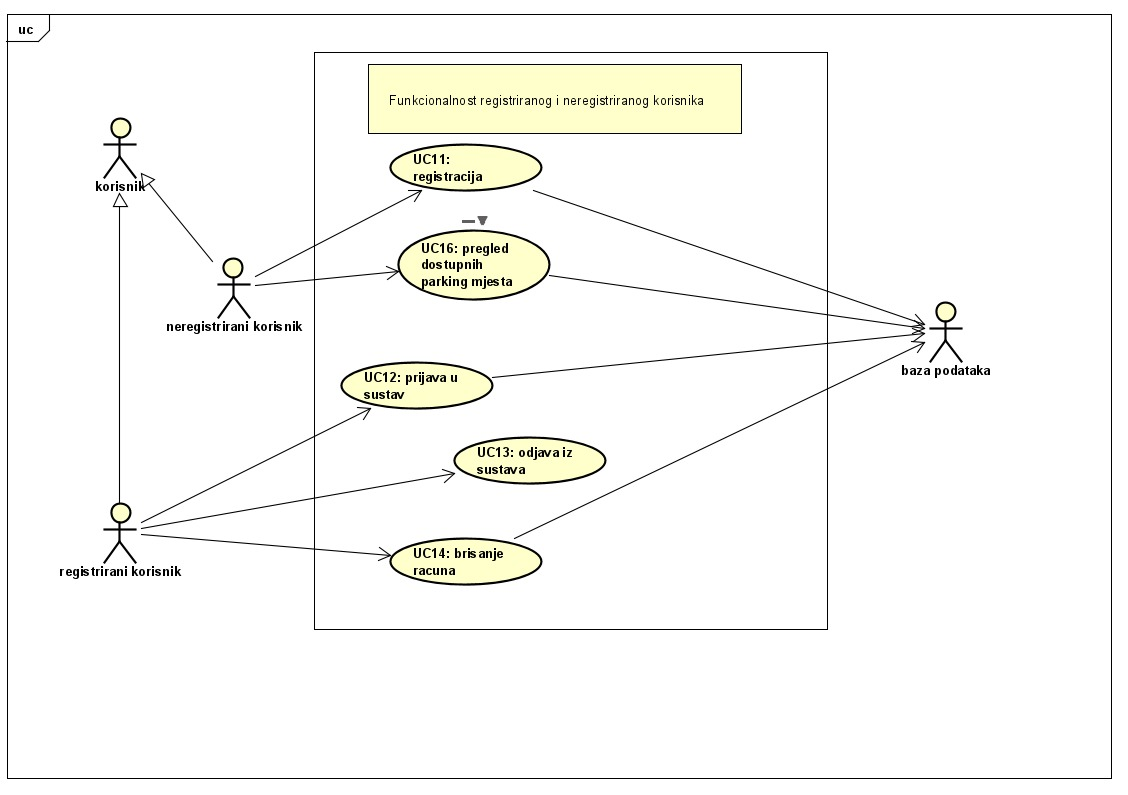
\includegraphics[width=\textwidth]{slika.jpeg} %veličina slike u odnosu na originalnu datoteku i pozicija slike
						\centering
						\caption{UC registrirani i neregistrirani korisnik}
						\label{fig:registrirani4312}
					\end{figure}
					
                    \begin{figure}[H]
						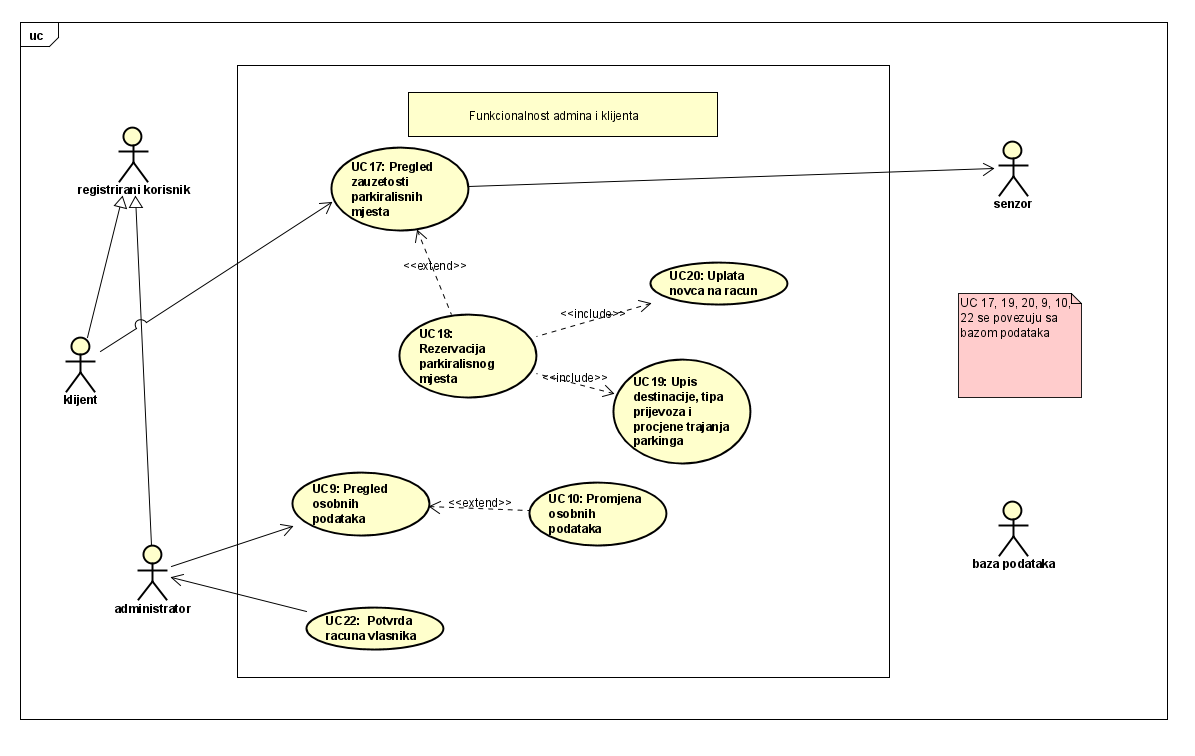
\includegraphics[width=\textwidth]{slike/klijent.PNG} %veličina slike u odnosu na originalnu datoteku i pozicija slike
						\caption{UC funkcionalnost klijenta i administratora}
						\label{fig:klijent}
					\end{figure}
				\eject		

				
			\subsection{Sekvencijski dijagrami}
				
				\textbf{\textit{dio 1. revizije}}\\
				
				\textit{Nacrtati sekvencijske dijagrame koji modeliraju najvažnije dijelove sustava (max. 4 dijagrama). Ukoliko postoji nedoumica oko odabira, razjasniti s asistentom. Uz svaki dijagram napisati detaljni opis dijagrama.}
				\eject
	
		\section{Ostali zahtjevi}
		
			\textbf{\textit{dio 1. revizije}}\\
		 
			 \textit{Nefunkcionalni zahtjevi i zahtjevi domene primjene dopunjuju funkcionalne zahtjeve. Oni opisuju \textbf{kako se sustav treba ponašati} i koja \textbf{ograničenja} treba poštivati (performanse, korisničko iskustvo, pouzdanost, standardi kvalitete, sigurnost...). Primjeri takvih zahtjeva u Vašem projektu mogu biti: podržani jezici korisničkog sučelja, vrijeme odziva, najveći mogući podržani broj korisnika, podržane web/mobilne platforme, razina zaštite (protokoli komunikacije, kriptiranje...)... Svaki takav zahtjev potrebno je navesti u jednoj ili dvije rečenice.}
			 
			 
			 
	
	\chapter{Arhitektura i dizajn sustava}


Sve web aplikacije sastavljene su od klijentske strane(eng.frontend) i od serverske strane(eng.backend). Kod u klijentskoj strani je pisan u HTML, CSS i JS i on se izvodi u web pregledniku. Dok serverska strana se sastoji od poslovne logike i koda koji odgovara na HTTP zahtjeve. Kod na serverskoj strani može biti pisan u Javi, PHP, Python, itd.



\begin{figure}[H]
	
	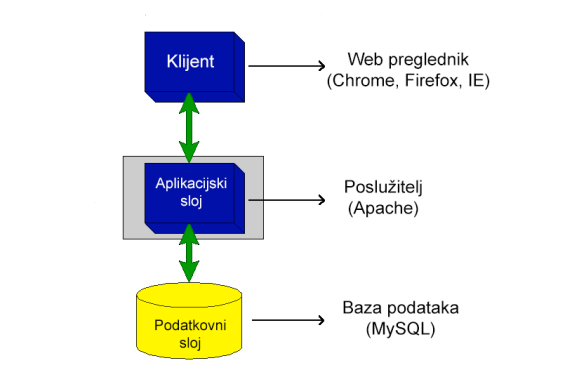
\includegraphics[width=\textwidth]{slike/webAplikacija.png} %veličina slike u odnosu na originalnu datoteku i pozicija slike
	\centering
	\caption{Arhitektura web aplikacije}
	\label{fig:arhitekturaWebApp}
\end{figure}
Web aplikacije podijeljene su na tri glavna sloja:

\begin{itemize}
	\item \textbf{Prvi sloj predstavlja prezentacijski sloj}, to je korisničko sučelje i komunikacijski sloj aplikacije gdje korisnik stupa u interakciju s aplikacijom. Glavna svrha prezentacijskog sloja je prikazivanje i prikupljanje informacija od korisnika.
	\item\textbf{Drugi sloj predstavlja aplikacijski sloj}, je glavni sloj web aplikacije. U ovom sloju se informacije prikupljene u prezentacijskom sloju obrađuju korištenjem poslovne logike. Te se također u ovom sloju dohvaćaju unose i izmjenjuju podatci koji se nalaze u podatkovnom sloju
	\item\textbf{Treći sloj je podatkovni sloj}, ili baza podataka je sloj u kojem se pohranjuju podatci koje koristi o obrađuje web aplikacija i u kojem se pristupa istim.
\end{itemize} 

Svi slojevi međusobno komuniciraju preko standardiziranih Internetskih protokola, kojih se prilikom razvoja 
aplikacija treba pridržavati.Glavne prednosti razvijanja aplikacija u tri sloja su:
\begin{itemize}
	\item Svaki sloj može biti napravljen u različitom programskom jeziku i okruženju.
	\item Svaki sloj može biti pokrenut na vlastitom serveru sto znači da slojevi ne ovise jedan o drugom.
	\item Brži razvoj aplikacije zato sto se svaki sloj može razvijati istovremeno.
	\item Poboljšana sigurnost zato sto možemo vršiti provjeru nad upitima i podatcima na tri razine i zbog toga što korisnik ne radi direktno sa SQL serverom.
\end{itemize}
Programski jezik kojeg smo odabrali za izradu naše web aplikacije je Java zajedno s Spring Boot-om i Thymeleaf-om. 
Odabrano razvojno okruženje je IntelliJ IDEA. Arhitektura sustava temeljiti  će se na MVC 
(Model-View-Controller) konceptu. MVC koncept podržan je od strane Spring Boot radnog okvira i kao takav ima gotove predloške koji nam olakšavaju razvoj web aplikacije.
MVC koncept sastoji se od:
\begin{itemize}
	\item \textbf{Model} - Komponenta Model sadrzi cijelu logiku vezanu za podatke s kojom korisnik radi. To mogu biti podatci koji se prenose između komponenti View i Controler ili bilo koje druge podatke vezane za poslovnu logiku.
	\item \textbf{View} - Komponenta View koristi se za svu logiku korisničkog sučelja aplikacije.  Na primjer, korisnički prikaz uključivat će sve komponente korisničkog sučelja kao što su tekstualni okviri, padajući izbornik itd. s kojima je u interakciji krajnji korisnik.
	\item \textbf{Controller} - Kontroleri djeluju kao sučelje između komponenti Modela i Viewa za obradu sve poslovne logike i dolaznih zahtjeva, manipuliranje podacima pomoću komponente Model i interakciju s Viewsima kako bi prikazali konačni izlaz.
\end{itemize} 
\eject


\section{Baza podataka}


Za našu web aplikaciju koristit ćemo relacijsku bazu podataka. Relacijska model baze podataka se sastoji od više tablica podataka takozvanih relacija. Svaka relacija ima svoje ime koje je jedinstveno u toj bazi podataka i koristimo ga za razlikovanje relacija u jednoj bazi podataka. Svaka relacija ima stupce koji sadrže vrijednost nekog atributa. Atribut ima svoje ime po kojem ga razlikujemo od drugih atributa u toj relaciji. Svaka tablica ima jedan ili više jednistvenih atributa ili skup atributa koji je jedinstven koji se koristi kao primarni ključ tablice. Entiteti u našoj bazi podataka su:

\begin{itemize}
	\item \textbf{Korisnik}(usertable)
	\item \textbf{Voditelj parkinga}(parkingowner)
	\item \textbf{Klijent}(client)
	\item \textbf{Rezervacija}(clientreservation)
	\item \textbf{Parkiralište}(parking)
	\item \textbf{Parkirališno mjesto}(parkingspot)
	\item \textbf{Zauzetost parkirnog mjesta}(parkingspotoccupancy)
\end{itemize}



\subsection{Opis tablica}


\textbf{Korisnik}  Ovaj entitet sadrži sve važne informacije o korisniku aplikacije. Sadrži atribute: identifikator korisnika, korisničko ime, ime, prezime, email korisnika, lozinku, tip korisnika aplikacije i oznaku je li administrator potvrdio taj korisnički račun. Ovaj entitet ima dvije specijalizacije na klijenta i voditelja parkinga.
\begin{longtblr}[
	label=none,
	entry=none
	]{
		width = \textwidth,
		colspec={|X[6,l]|X[6, l]|X[20, l]|}, 
		rowhead = 1,
	} %definicija širine tablice, širine stupaca, poravnanje i broja redaka naslova tablice
	\hline \multicolumn{3}{|c|}{\textbf{Korisnik(usertable)}}	 \\ \hline[3pt]
	\SetCell{LightGreen}userid & INT	&  	Jedinstveni identifikator korisnika  	\\ \hline
	username	& VARCHAR &   Korisničko ime	\\ \hline 
	userfirstname & VARCHAR & Ime korisnika  \\ \hline 
	usersurename & VARCHAR	&  Prezime korisnika		\\ \hline 
	useremail & VARCHAR & Email korinika \\ \hline
	temppassword & VARCHAR & Privremena lozinka \\ \hline
	usertype & VARCHAR & Tip korisnika aplikacije (voditelj ili klijent)\\\hline
	confirmed & BOOLEAN & Varijabla koja pokazuje je li korisnik potvrđen od strane administratora \\\hline
\end{longtblr}

\textbf{Voditelj parkirališta}  Ovaj entitet je specijalizacija entiteta korisnik on sadrži dodatne atribute: iban i poveznicu na sliku osobne iskaznice. Povezan je sa parkiralištem vezom n naprema n.
\begin{longtblr}[
	label=none,
	entry=none
	]{
		width = \textwidth,
		colspec={|X[6,l]|X[6, l]|X[20, l]|}, 
		rowhead = 1,
	} %definicija širine tablice, širine stupaca, poravnanje i broja redaka naslova tablice
	\hline \multicolumn{3}{|c|}{\textbf{Voditelj parkirališta(parkingowner)}}\\ \hline[3pt]
	\SetCell{LightGreen}userid & INT	&  	Jedinstveni identifikator korisnika  	\\ \hline
	iban	& CHARACTER &   IBAN vlasnika parkinga	\\ \hline 
	idpicture & VARCHAR &  Poveznica na sliku osobne iskaznice \\ \hline 
\end{longtblr}

\textbf{Klijent}  Ovaj entitet je specijalizacija entiteta korisnik on sadrži dodatni atribut stanje računa klijenta. Povezan je sa entitetom rezervacija vezom n naprema n.
\begin{longtblr}[
	label=none,
	entry=none
	]{
		width = \textwidth,
		colspec={|X[6,l]|X[6, l]|X[20, l]|}, 
		rowhead = 1,
	} %definicija širine tablice, širine stupaca, poravnanje i broja redaka naslova tablice
	\hline \multicolumn{3}{|c|}{\textbf{Klijent(client)}}\\ \hline[3pt]
	\SetCell{LightGreen}userid & INT	&  	Jedinstveni identifikator korisnika  	\\ \hline
	walletbalance	& NUMERIC &   Stanje računa klijenta	\\ \hline 
\end{longtblr}

\textbf{Parkiralište}  Ovaj entitet sadrži sve bitne informacije o parkiralištu. Atributi su mu: korisnički id voditelja parkirališta, ime parkinga, poveznica na sliku parkinga, cijena parkinga po satu i opis parkirališta. Povezan je sa voditeljem parkiralista vezom n naprema n i sa parkirališnim mjestom vezom n naprema n. 
\begin{longtblr}[
	label=none,
	entry=none
	]{
		width = \textwidth,
		colspec={|X[6,l]|X[6, l]|X[20, l]|}, 
		rowhead = 1,
	} %definicija širine tablice, širine stupaca, poravnanje i broja redaka naslova tablice
	\hline \multicolumn{3}{|c|}{\textbf{Parkiralište(parking)}}	 \\ \hline[3pt]
	\SetCell{LightGreen}userid & INT	&  	Jedinstveni identifikator voditelja parkinga  	\\ \hline
	parkingname	& VARCHAR &   Ime parkirališta	\\ \hline 
	parkingphoto & VARCHAR &  Poveznica na sliku parkirališta \\ \hline 
	hourlyprice & VARCHAR	&  Cijena parkiranja po satu		\\ \hline 
	description & VARCHAR &   Opis parkirališta	\\ \hline 
\end{longtblr}

\textbf{Parkirališno mjesto}  Ovaj entitet sadrži sve bitne informacije o parkirališnom mjestu. Atributi su mu: korisnički id voditelja parkirališta, broj parkirališnog mjesta na parkiralištu, tip parkirališnog mjesta, mogućnost rezervacije te x i y koordinate za 4 točke koje označavaju granice parkirališnog mjesta. Povezan je vezon n naprema n sa parkiralištem i rezervacijom a vezom 1 naprema n sa zauzetosti parkirališnog mjesta.
\begin{longtblr}[
	label=none,
	entry=none
	]{
		width = \textwidth,
		colspec={|X[10,l]|X[6, l]|X[20, l]|}, 
		rowhead = 1,
	} %definicija širine tablice, širine stupaca, poravnanje i broja redaka naslova tablice
	\hline \multicolumn{3}{|c|}{\textbf{Parkirališno mjesto(parkingspot)}}	 \\ \hline[3pt]
	\SetCell{LightGreen}userid & INT	&  	Jedinstveni identifikator voditelja parkinga  	\\ \hline
	\SetCell{LightGreen}parkingspotnumber & INT	&  	Broj parkirališnog mjesta na parkiralištu  	\\ \hline
	parkingspottype	& VARCHAR &   Vrsta parkirališnog mjesta(Za automobile ili za bicikle)	\\ \hline 
	canbereserved & BOOLEAN & Mogućnost rezerviranja parkirališnog mjesta  \\ \hline 
	pointx1 & NUMERIC & Koordinata x prve točke parkirnog mjesta\\\hline
	pointy1 & NUMERIC & Koordinata y prve točke parkirnog mjesta\\\hline
	pointx2 & NUMERIC & Koordinata x druge točke parkirnog mjesta\\\hline
	pointy2 & NUMERIC & Koordinata y druge točke parkirnog mjesta\\\hline
	pointx3 & NUMERIC & Koordinata x treće točke parkirnog mjesta\\\hline
	pointy3 & NUMERIC & Koordinata y treće točke parkirnog mjesta\\\hline
	pointx4 & NUMERIC & Koordinata x četvrte točke parkirnog mjesta\\\hline
	pointy4 & NUMERIC & Koordinata y četvrte točke parkirnog mjesta\\\hline
\end{longtblr}

\textbf{Zauzetost parkirališnog mjesta}  Ovaj entitet sadrži informacije koje se koriste za statističku analizu zauzetosti parkirališnog mjesta. Atributi su mu: korisnički id voditelja parkirališta, broj parkirališnog mjesta na parkiralištu, vrijeme od, vrijeme do i zauzetost u tom razdoblju. Povezan je vezom n naprema 1 sa parkirališnim mjestom.
\begin{longtblr}[
	label=none,
	entry=none
	]{
		width = \textwidth,
		colspec={|X[10,l]|X[6, l]|X[20, l]|}, 
		rowhead = 1,
	} %definicija širine tablice, širine stupaca, poravnanje i broja redaka naslova tablice
	\hline \multicolumn{3}{|c|}{\textbf{Zauzetost parkirnog mjesta(parkingspotoccupancy)}}	 \\ \hline[3pt]
	\SetCell{LightGreen}userid & INT	&  	Jedinstveni identifikator voditelja parkinga  	\\ \hline
	\SetCell{LightGreen}parkingspotnumber & INT	&  	Broj parkirnog mjesta na parkiralištu  	\\ \hline
	\SetCell{LightGreen}datefrom & TIMESTAMP	&  	Početak zauzetosti parkirališnog mjesta	\\ \hline
	dateto	& TIMESTAMP &  	Kraj zauzetosti parkirališnog mjesta	 	\\ \hline 
	occupancy & BOOLEAN  &  Varijabla koja nam govori da li je parkirališno mjesto bilo zauzeto \\ \hline 
\end{longtblr}
\eject
\textbf{Rezervacija}  Ovaj entitet sadrži informacije o rezervacijama parkirališnih mjesta. Sadrži atribute: jedinstveni identifikator klijenta, vrijeme početka rezervacije, jedinstveni identifikator voditelja parkinga, broj parkirnog mjesta na parkiralištu, duljina rezervacije i varijablu koja nam govori je li rezervacija ponavljajuća. Povezan je vezon n naprema n sa klijentom i sa parkirališnim mjestom.
\begin{longtblr}[
	label=none,
	entry=none
	]{
		width = \textwidth,
		colspec={|X[10,l]|X[6, l]|X[20, l]|}, 
		rowhead = 1,
	} %definicija širine tablice, širine stupaca, poravnanje i broja redaka naslova tablice
	\hline \multicolumn{3}{|c|}{\textbf{Rezervacija(clientreservation)}	 }\\ \hline[3pt]
	\SetCell{LightGreen}userid & INT	&  	Jedinstveni identifikator klijenta 	\\ \hline
	\SetCell{LightGreen}timeofstart & TIMESTAMP	&  	Vrijeme početka rezervacije  	\\ \hline
	\SetCell{LightBlue}userid & INT	&  	Jedinstveni identifikator voditelja parkinga  	\\ \hline
	\SetCell{LightBlue}parkingspotnumber & INT	&  	Broj parkirnog mjesta na parkiralištu  	\\ \hline
	duration & INT & Duljina rezervacije\\ \hline 
	reccuring & BOOLEAN & Varijabla koja definira je li rezervacija ponavljajuća \\\hline
\end{longtblr}

\subsection{Dijagram baze podataka}


\begin{figure}[H]
	
	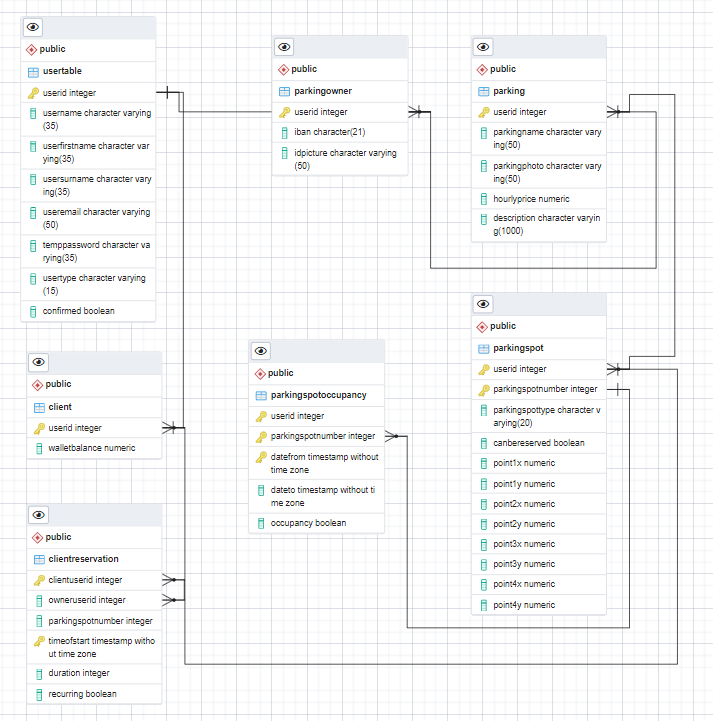
\includegraphics[width=\textwidth]{slike/db.png} %veličina slike u odnosu na originalnu datoteku i pozicija slike
	\centering
	\caption{E-R dijagram baze podataka}
	\label{fig:dijagramBP}
\end{figure}

\eject



\section{Dijagram razreda}

\textit{Potrebno je priložiti dijagram razreda s pripadajućim opisom. Zbog preglednosti je moguće dijagram razlomiti na više njih, ali moraju biti grupirani prema sličnim razinama apstrakcije i srodnim funkcionalnostima.}\\

\textbf{\textit{dio 1. revizije}}\\

\textit{Prilikom prve predaje projekta, potrebno je priložiti potpuno razrađen dijagram razreda vezan uz \textbf{generičku funkcionalnost} sustava. Ostale funkcionalnosti trebaju biti idejno razrađene u dijagramu sa sljedećim komponentama: nazivi razreda, nazivi metoda i vrste pristupa metodama (npr. javni, zaštićeni), nazivi atributa razreda, veze i odnosi između razreda.}\\

\textbf{\textit{dio 2. revizije}}\\			

\textit{Prilikom druge predaje projekta dijagram razreda i opisi moraju odgovarati stvarnom stanju implementacije}



\eject

\section{Dijagram stanja}


\textbf{\textit{dio 2. revizije}}\\

\textit{Potrebno je priložiti dijagram stanja i opisati ga. Dovoljan je jedan dijagram stanja koji prikazuje \textbf{značajan dio funkcionalnosti} sustava. Na primjer, stanja korisničkog sučelja i tijek korištenja neke ključne funkcionalnosti jesu značajan dio sustava, a registracija i prijava nisu. }


\eject 

\section{Dijagram aktivnosti}

\textbf{\textit{dio 2. revizije}}\\

\textit{Potrebno je priložiti dijagram aktivnosti s pripadajućim opisom. Dijagram aktivnosti treba prikazivati značajan dio sustava.}

\eject
\section{Dijagram komponenti}

\textbf{\textit{dio 2. revizije}}\\

\textit{Potrebno je priložiti dijagram komponenti s pripadajućim opisom. Dijagram komponenti treba prikazivati strukturu cijele aplikacije.}
	\chapter{Implementacija i korisničko sučelje}
		
		
		\section{Korištene tehnologije i alati}
		
			\textbf{\textit{dio 2. revizije}}
			
			 \textit{Detaljno navesti sve tehnologije i alate koji su primijenjeni pri izradi dokumentacije i aplikacije. Ukratko ih opisati, te navesti njihovo značenje i mjesto primjene. Za svaki navedeni alat i tehnologiju je potrebno \textbf{navesti internet poveznicu} gdje se mogu preuzeti ili više saznati o njima}.
			
			
			\eject 
		
	
		\section{Ispitivanje programskog rješenja}
			
			\textbf{\textit{dio 2. revizije}}\\
			
			 \textit{U ovom poglavlju je potrebno opisati provedbu ispitivanja implementiranih funkcionalnosti na razini komponenti i na razini cijelog sustava s prikazom odabranih ispitnih slučajeva. Studenti trebaju ispitati temeljnu funkcionalnost i rubne uvjete.}
	
			
			\subsection{Ispitivanje komponenti}
			\textit{Potrebno je provesti ispitivanje jedinica (engl. unit testing) nad razredima koji implementiraju temeljne funkcionalnosti. Razraditi \textbf{minimalno 6 ispitnih slučajeva} u kojima će se ispitati redovni slučajevi, rubni uvjeti te izazivanje pogreške (engl. exception throwing). Poželjno je stvoriti i ispitni slučaj koji koristi funkcionalnosti koje nisu implementirane. Potrebno je priložiti izvorni kôd svih ispitnih slučajeva te prikaz rezultata izvođenja ispita u razvojnom okruženju (prolaz/pad ispita). }
			
			
			
			\subsection{Ispitivanje sustava}
			
			 \textit{Potrebno je provesti i opisati ispitivanje sustava koristeći radni okvir Selenium\footnote{\url{https://www.seleniumhq.org/}}. Razraditi \textbf{minimalno 4 ispitna slučaja} u kojima će se ispitati redovni slučajevi, rubni uvjeti te poziv funkcionalnosti koja nije implementirana/izaziva pogrešku kako bi se vidjelo na koji način sustav reagira kada nešto nije u potpunosti ostvareno. Ispitni slučaj se treba sastojati od ulaza (npr. korisničko ime i lozinka), očekivanog izlaza ili rezultata, koraka ispitivanja i dobivenog izlaza ili rezultata.\\ }
			 
			 \textit{Izradu ispitnih slučajeva pomoću radnog okvira Selenium moguće je provesti pomoću jednog od sljedeća dva alata:}
			 \begin{itemize}
			 	\item \textit{dodatak za preglednik \textbf{Selenium IDE} - snimanje korisnikovih akcija radi automatskog ponavljanja ispita	}
			 	\item \textit{\textbf{Selenium WebDriver} - podrška za pisanje ispita u jezicima Java, C\#, PHP koristeći posebno programsko sučelje.}
			 \end{itemize}
		 	\textit{Detalji o korištenju alata Selenium bit će prikazani na posebnom predavanju tijekom semestra.}
			
			\eject 
		
		
		\section{Dijagram razmještaja}
			
			\textbf{\textit{dio 2. revizije}}
			
			 \textit{Potrebno je umetnuti \textbf{specifikacijski} dijagram razmještaja i opisati ga. Moguće je umjesto specifikacijskog dijagrama razmještaja umetnuti dijagram razmještaja instanci, pod uvjetom da taj dijagram bolje opisuje neki važniji dio sustava.}
			
			\eject 
		
		\section{Upute za puštanje u pogon}
		
			\textbf{\textit{dio 2. revizije}}\\
		
			 \textit{U ovom poglavlju potrebno je dati upute za puštanje u pogon (engl. deployment) ostvarene aplikacije. Na primjer, za web aplikacije, opisati postupak kojim se od izvornog kôda dolazi do potpuno postavljene baze podataka i poslužitelja koji odgovara na upite korisnika. Za mobilnu aplikaciju, postupak kojim se aplikacija izgradi, te postavi na neku od trgovina. Za stolnu (engl. desktop) aplikaciju, postupak kojim se aplikacija instalira na računalo. Ukoliko mobilne i stolne aplikacije komuniciraju s poslužiteljem i/ili bazom podataka, opisati i postupak njihovog postavljanja. Pri izradi uputa preporučuje se \textbf{naglasiti korake instalacije uporabom natuknica} te koristiti što je više moguće \textbf{slike ekrana} (engl. screenshots) kako bi upute bile jasne i jednostavne za slijediti.}
			
			
			 \textit{Dovršenu aplikaciju potrebno je pokrenuti na javno dostupnom poslužitelju. Studentima se preporuča korištenje neke od sljedećih besplatnih usluga: \href{https://aws.amazon.com/}{Amazon AWS}, \href{https://azure.microsoft.com/en-us/}{Microsoft Azure} ili \href{https://www.heroku.com/}{Heroku}. Mobilne aplikacije trebaju biti objavljene na F-Droid, Google Play ili Amazon App trgovini.}
			
			
			\eject 
	\chapter{Zaključak i budući rad}
		
		\textbf{\textit{dio 2. revizije}}\\
		
		 \textit{U ovom poglavlju potrebno je napisati osvrt na vrijeme izrade projektnog zadatka, koji su tehnički izazovi prepoznati, jesu li riješeni ili kako bi mogli biti riješeni, koja su znanja stečena pri izradi projekta, koja bi znanja bila posebno potrebna za brže i kvalitetnije ostvarenje projekta i koje bi bile perspektive za nastavak rada u projektnoj grupi.}
		
		 \textit{Potrebno je točno popisati funkcionalnosti koje nisu implementirane u ostvarenoj aplikaciji.}
		
		\eject 
	\chapter*{Popis literature}
		\addcontentsline{toc}{chapter}{Popis literature}
	 	
 		\textbf{\textit{Kontinuirano osvježavanje}}
	
		\textit{Popisati sve reference i literaturu koja je pomogla pri ostvarivanju projekta.}
		
		
		\begin{enumerate}
			
			
			\item  Programsko inženjerstvo, FER ZEMRIS, \url{http://www.fer.hr/predmet/proinz}
			
			\item  I. Sommerville, "Software engineering", 8th ed, Addison Wesley, 2007.
			
			\item  T.C.Lethbridge, R.Langaniere, "Object-Oriented Software Engineering", 2nd ed. McGraw-Hill, 2005.
			
			\item  I. Marsic, Software engineering book``, Department of Electrical and Computer Engineering, Rutgers University, \url{http://www.ece.rutgers.edu/~marsic/books/SE}
			
			\item  The Unified Modeling Language, \url{https://www.uml-diagrams.org/}
			
			\item  Astah Community, \url{http://astah.net/editions/uml-new}
		\end{enumerate}
		
		 
	
	
	\begingroup
	\renewcommand*\listfigurename{Indeks slika i dijagrama}
	%\renewcommand*\listtablename{Indeks tablica}
	%\let\clearpage\relax
	\listoffigures
	%\vspace{10mm}
	%\listoftables
	\endgroup
	\addcontentsline{toc}{chapter}{Indeks slika i dijagrama}


	
	\eject 
		
	\chapter*{Dodatak: Prikaz aktivnosti grupe}
		\addcontentsline{toc}{chapter}{Dodatak: Prikaz aktivnosti grupe}
		
		\section*{Dnevnik sastajanja}
		
		\textbf{\textit{Kontinuirano osvježavanje}}\\
		
		
		\begin{packed_enum}
				\item  sastanak
			
			\item[] \begin{packed_item}
				\item Datum: u ovom formatu: 14.10.2021.
				\item Prisustvovali: M.Barbir, M.Ivić, F.Bura, M.Žura, M.Puharić, L.Gjurić, Z.Ravlić
				\item Teme sastanka:
				\begin{packed_item}
					\item  Prvi sastanak tima
					\item  Formiranje grupe
				\end{packed_item}
			\end{packed_item}
			\item  sastanak
		
		\item[] \begin{packed_item}
			\item Datum: u ovom formatu: 25.10.2021.
			\item Prisustvovali: M.Barbir, M.Ivić, F.Bura, M.Žura, M.Puharić, L.Gjurić, Z.Ravlić
			\item Teme sastanka:
			\begin{packed_item}
				\item  Raspodjela na frontend i backend
				\item  Raspodjela rada na dokumentaciji
			\end{packed_item}
		\end{packed_item}
			\item  sastanak
			
			\item[] \begin{packed_item}
				\item Datum: u ovom formatu: 2.11.2021.
				\item Prisustvovali: M.Barbir, M.Ivić, F.Bura, M.Žura, M.Puharić, L.Gjurić, Z.Ravlić
				\item Teme sastanka:
				\begin{packed_item}
					\item  Rasprava o stanju na projektu
				\end{packed_item}
			\end{packed_item}
			
			\item  sastanak
			\item[] \begin{packed_item}
				\item Datum: u ovom formatu: 15.11.2021.
				\item Prisustvovali: M.Barbir, M.Ivić, F.Bura, M.Žura, M.Puharić, L.Gjurić, Z.Ravlić
				\item Teme sastanka:
				\begin{packed_item}
					\item  Rasprava o stanju na projektu
					\item  Pregled dokumentacije
					\item  Dogovor o deployju aplikacije 
				\end{packed_item}
			\end{packed_item}
			
			%
			
		\end{packed_enum}
		
		\eject
		\section*{Tablica aktivnosti}
		
			\textbf{\textit{Kontinuirano osvježavanje}}\\
			

			\begin{longtblr}[
					label=none,
				]{
					vlines,hlines,
					width = \textwidth,
					colspec={X[7, l]X[1, c]X[1, c]X[1, c]X[1, c]X[1, c]X[1, c]X[1, c]}, 
					vline{1} = {1}{text=\clap{}},
					hline{1} = {1}{text=\clap{}},
					rowhead = 1,
				} 
				\multicolumn{1}{c|}{} & \multicolumn{1}{c|}{\rotatebox{90}{\textbf{Marko Barbir}}} & \multicolumn{1}{c|}{\rotatebox{90}{\textbf{Luka Gjuric }}} &	\multicolumn{1}{c|}{\rotatebox{90}{\textbf{Marko Žura }}} & \multicolumn{1}{c|}{\rotatebox{90}{\textbf{Filip Bura }}} &	\multicolumn{1}{c|}{\rotatebox{90}{\textbf{Marin Puharić }}} & \multicolumn{1}{c|}{\rotatebox{90}{\textbf{Zvonimir Ravlić }}} &	\multicolumn{1}{c|}{\rotatebox{90}{\textbf{Mate Ivić }}} \\  
<<<<<<< HEAD
<<<<<<< HEAD
				Upravljanje projektom 		&  &  &  6  &  &  & \\ 
				Opis projektnog zadatka 	&  &  &  5  &  &  & \\ 
=======
				Upravljanje projektom 		&  &  &  &  &  &  & \\ 
				Opis projektnog zadatka 	&  &  &  &  &  &  & \\ 
>>>>>>> parent of 61ddb3c (added: working hours)
				
				Funkcionalni zahtjevi       &  &  &  &  &  &  &  \\ 
				Opis pojedinih obrazaca 	&  &  &  &  &  &  &  \\ 
				Dijagram obrazaca 			&  &  &  &  &  &  &  \\ 
				Sekvencijski dijagrami 		&  &  &  &  &  &  &  \\ 
				Opis ostalih zahtjeva 		&  &  &  &  &  &  &  \\ 

				Arhitektura i dizajn sustava	 &  &  &  &  &  &  &  \\ 
				Baza podataka				&  &  &  &  &  &  &   \\ 
				Dijagram razreda 			&  &  &  &  &  &  &   \\ 
				Dijagram stanja				&  &  &  &  &  &  &  \\ 
				Dijagram aktivnosti 		&  &  &  &  &  &  &  \\ 
				Dijagram komponenti			&  &  &  &  &  &  &  \\ 
				Korištene tehnologije i alati 		&  &  &  &  &  &  &  \\ 
				Ispitivanje programskog rješenja 	&  &  &  &  &  &  &  \\ 
				Dijagram razmještaja			&  &  &  &  &  &  &  \\ 
				Upute za puštanje u pogon 		&  &  &  &  &  &  &  \\  
				Dnevnik sastajanja 			&  &  &  &  &  &  &  \\ 
				Zaključak i budući rad 		&  &  &  &  &  &  &  \\  
				Popis literature 			&  &  &  &  &  &  &  \\  
				&  &  &  &  &  &  &  \\ \hline 
				
				Izrada početne stranice 				&  &  &  &  &  &  &  \\  
				Izrada baze podataka	 			&  &  &  &  &  &  & \\  
				Sspajanje s bazom podataka 							&  &  &  &  &  &  &  \\ 
				Back end 							&  &  &  &  &  &  &  \\  
<<<<<<< HEAD
				Front end 							&  &  &  20  &  &  &\\ 
=======
				Upravljanje projektom 		&10  &  &  &  &  &  & \\ 
				Opis projektnog zadatka 	&0  &  &  &  &  &  & \\ 
				
				Funkcionalni zahtjevi       &2  &  &  &  &  &  &  \\ 
				Opis pojedinih obrazaca 	&1  &  &  &  &  &  &  \\ 
				Dijagram obrazaca 			&0  &  &  &  &  &  &  \\ 
				Sekvencijski dijagrami 		&0  &  &  &  &  &  &  \\ 
				Opis ostalih zahtjeva 		&0  &  &  &  &  &  &  \\ 

				Arhitektura i dizajn sustava	 &1  &  &  &  &  &  &  \\ 
				Baza podataka				&1  &  &  &  &  &  &   \\ 
				Dijagram razreda 			&0  &  &  &  &  &  &   \\ 
				Dijagram stanja				&0  &  &  &  &  &  &  \\ 
				Dijagram aktivnosti 		&0  &  &  &  &  &  &  \\ 
				Dijagram komponenti			&0  &  &  &  &  &  &  \\ 
				Korištene tehnologije i alati 		&0  &  &  &  &  &  &  \\ 
				Ispitivanje programskog rješenja 	&0  &  &  &  &  &  &  \\ 
				Dijagram razmještaja			&0  &  &  &  &  &  &  \\ 
				Upute za puštanje u pogon 		&0  &  &  &  &  &  &  \\  
				Dnevnik sastajanja 			&0.5  &  &  &  &  &  &  \\ 
				Zaključak i budući rad 		&0  &  &  &  &  &  &  \\  
				Popis literature 			&0  &  &  &  &  &  &  \\  \hline 
				
				Izrada početne stranice 				&10  &  &  &  &  &  &  \\  
				Izrada baze podataka	 			&5  &  &  &  &  &  & \\  
				Sspajanje s bazom podataka 							&3  &  &  &  &  &  &  \\ 
				Back end 							&60  &  &  &  &  &  &  \\  
				Front end							&30  &  &  &  &  &  &\\ 
			\end{longtblr}
					
					
		\eject
		\section*{Dijagrami pregleda promjena}
		
		\textbf{\textit{dio 2. revizije}}\\
		
		\textit{Prenijeti dijagram pregleda promjena nad datotekama projekta. Potrebno je na kraju projekta generirane grafove s gitlaba prenijeti u ovo poglavlje dokumentacije. Dijagrami za vlastiti projekt se mogu preuzeti s gitlab.com stranice, u izborniku Repository, pritiskom na stavku Contributors.}
		
	

\end{document} %naredbe i tekst nakon ove naredbe ne ulaze u izgrađen dokument 


